Fig.~\ref{fig:app} shows the running application, served on the same GPU used for evaluation. Each test used a
note that is not in the dataset, together with criteria that we wrote ourselves:
\begin{itemize}
\item a 67-year-old man with type~2 diabetes and stage~3 chronic kidney disease;
\item a hypothetical add-on therapy trial with three inclusion and four exclusion criteria.
\end{itemize}
The note is split into numbered sentences, and each criterion is decoded and displayed as soon as it finishes.
Each result card shows:
\begin{itemize}
\item the label, with both criterion types kept and all expert categories preserved;
\item the cited sentences, which are also highlighted in the note;
\item a rationale that passed the grounding check, or the deterministic template when it did not.
\end{itemize}
The overall outcome is shown together with the rule that produced it.

Invalid input is rejected with a field-level message and the user's draft is kept. This covers empty notes,
malformed NCT IDs and unknown labels. An unreachable ClinicalTrials.gov service or a model that is still
loading returns a clear message, not a stack trace.

The Inference Lab runs the no-cache, KV-cached and speculative decoders on the loaded model. For each run it
reports timing, token equality and draft acceptance, and it also runs the attention check against a float64
ground truth.

\begin{figure*}[t]
\centering
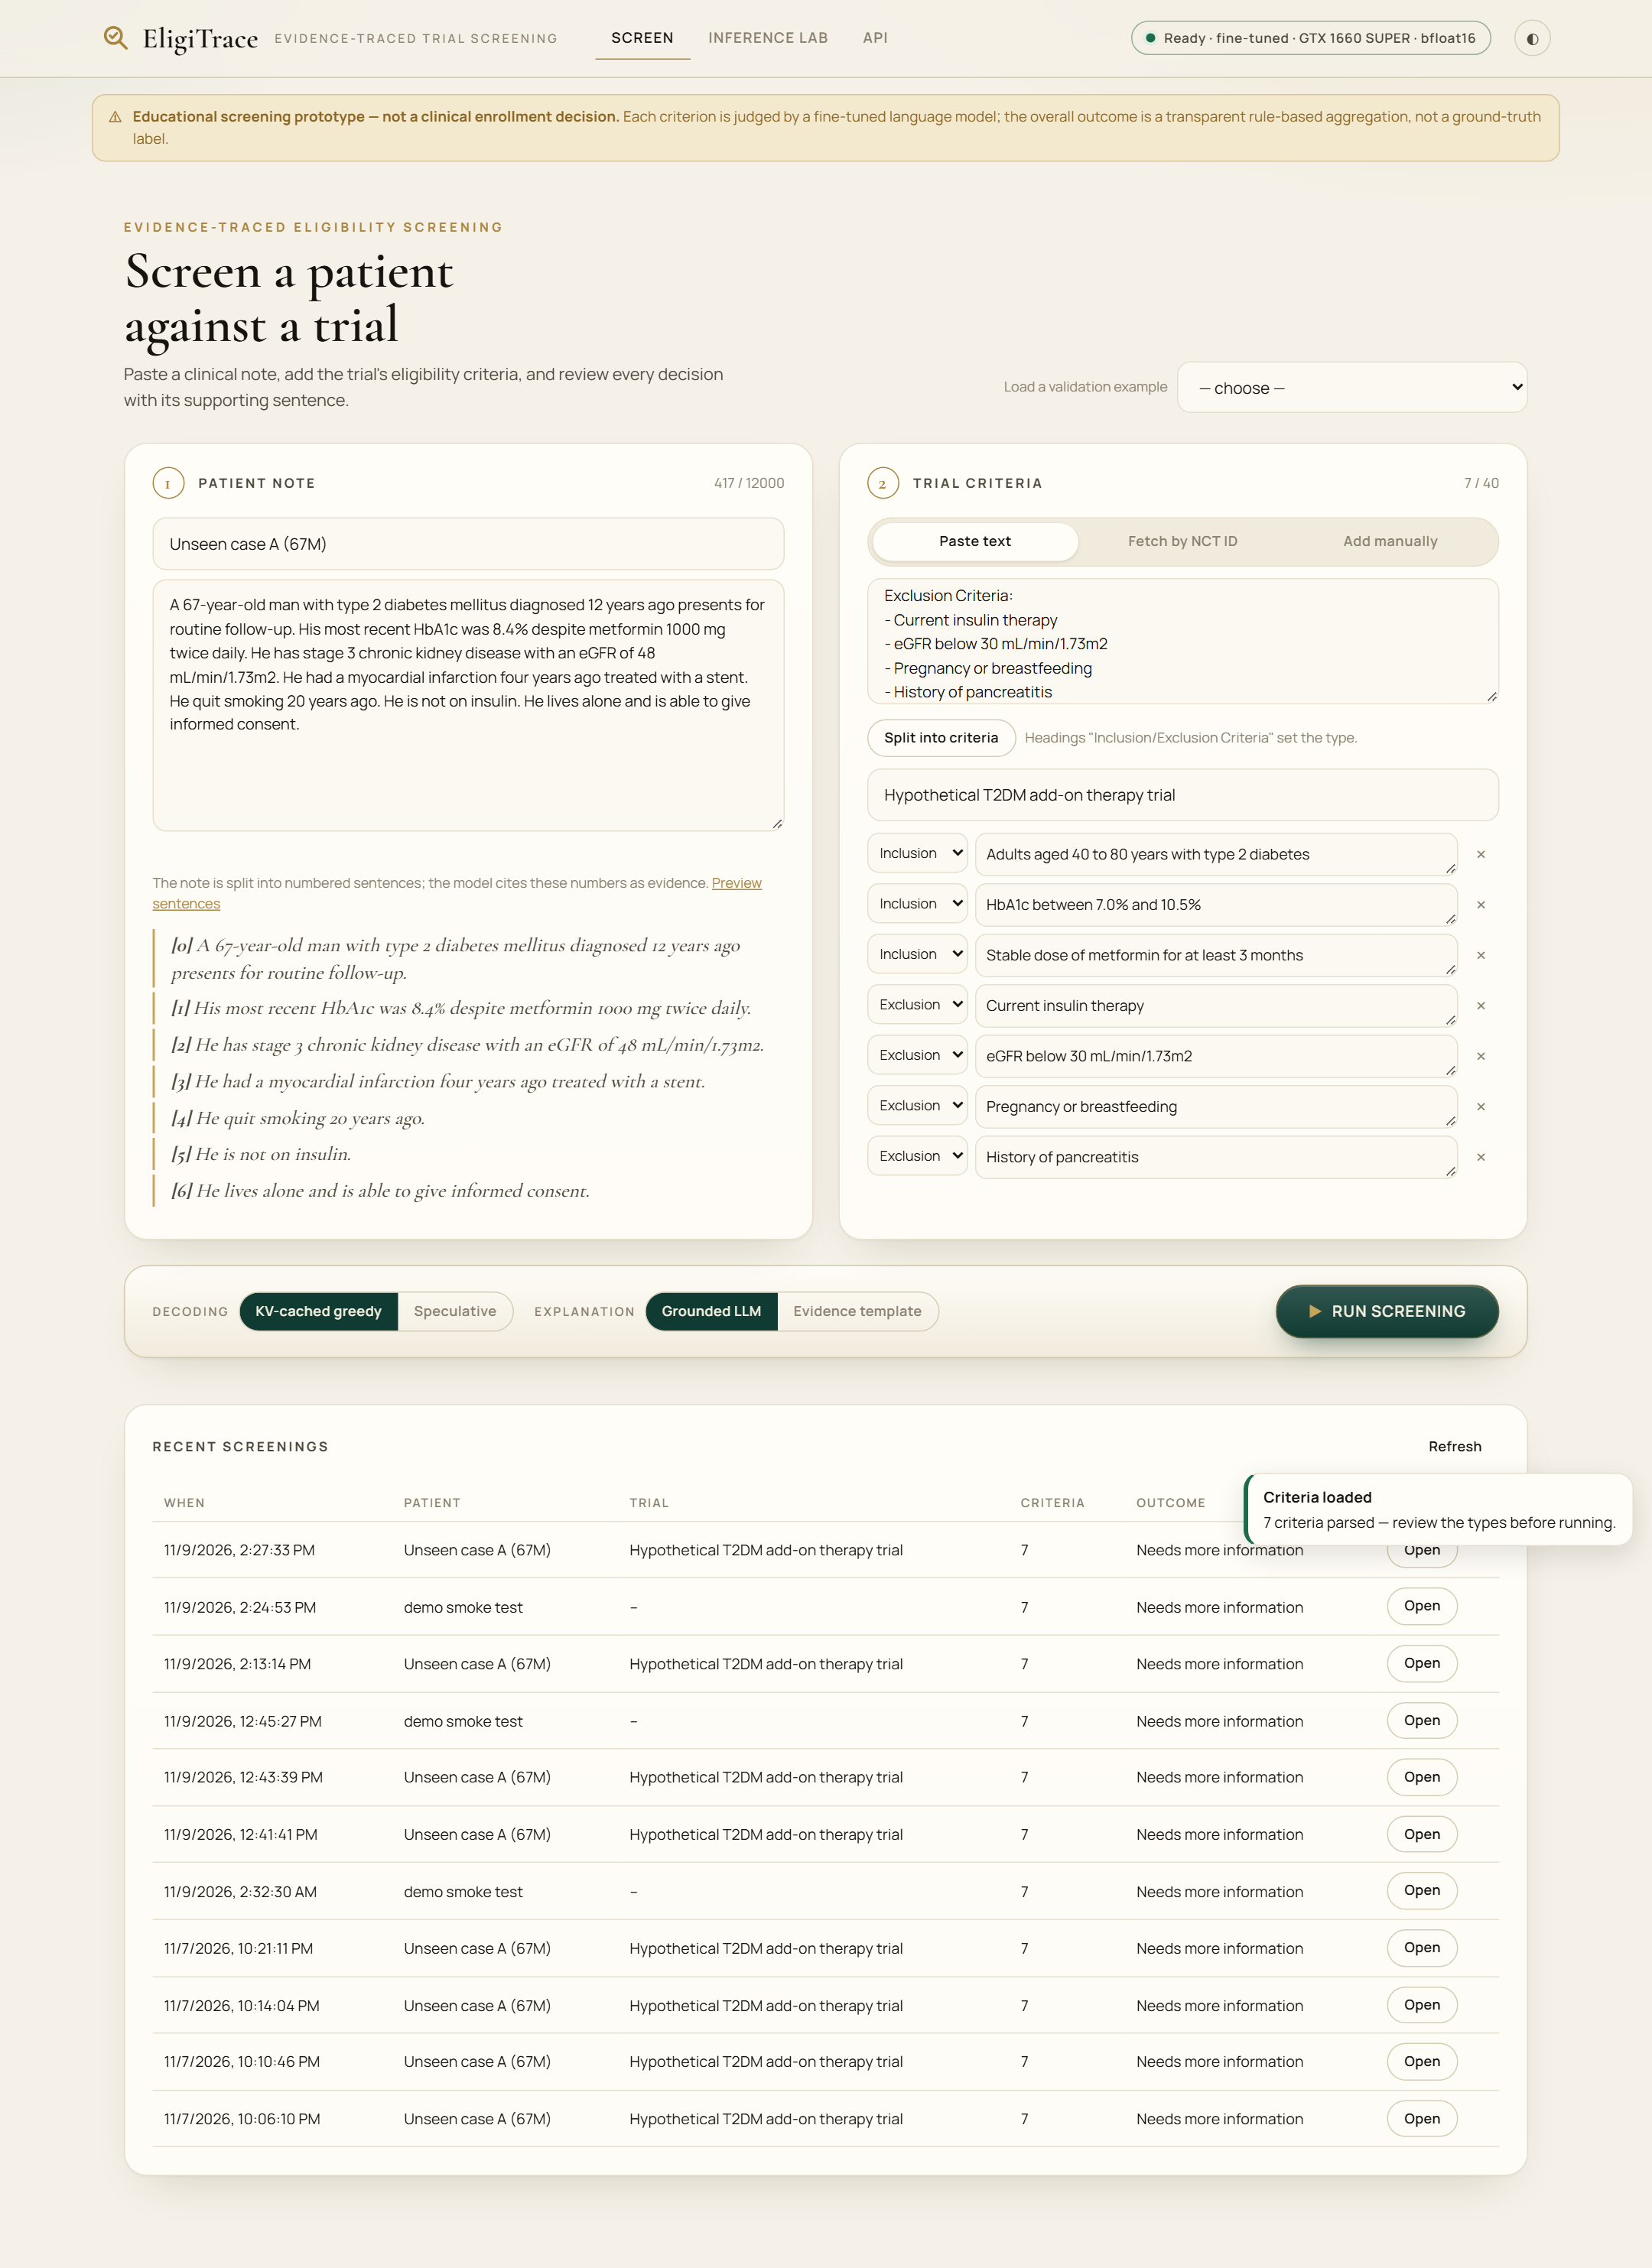
\includegraphics[width=0.49\linewidth]{screens/02_input.png}\hfill
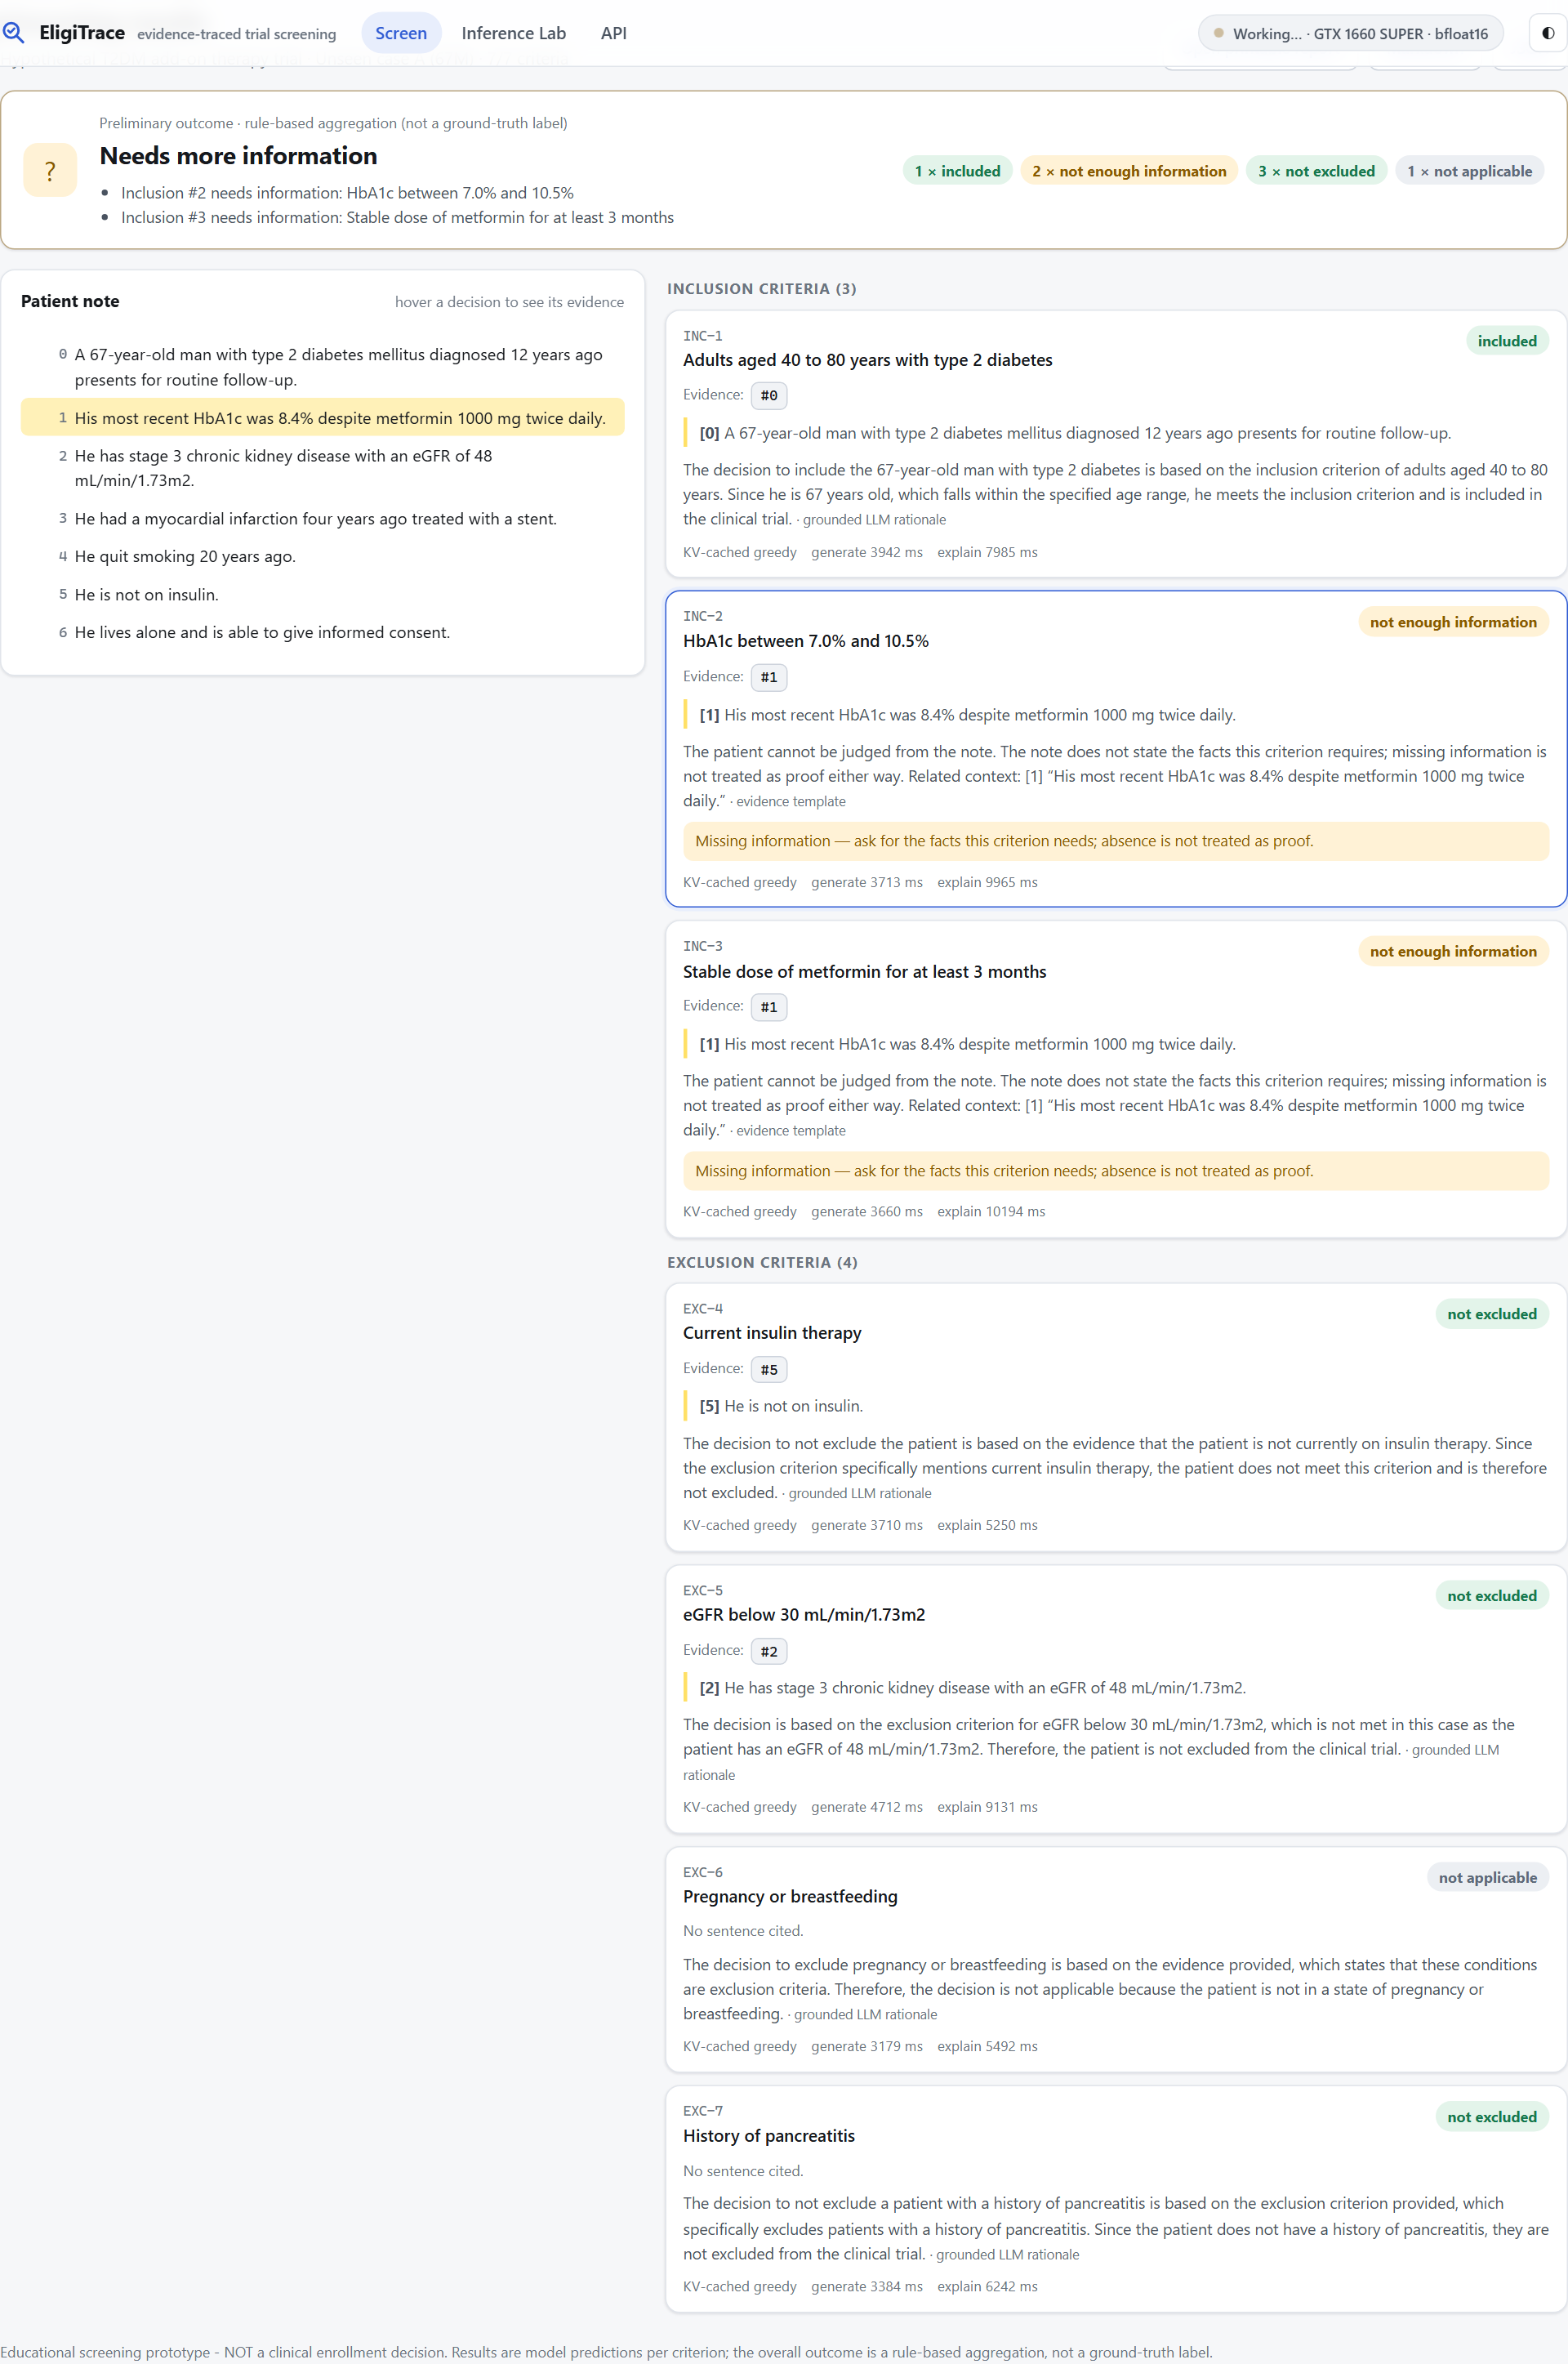
\includegraphics[width=0.49\linewidth]{screens/03_results.png}\\[4pt]
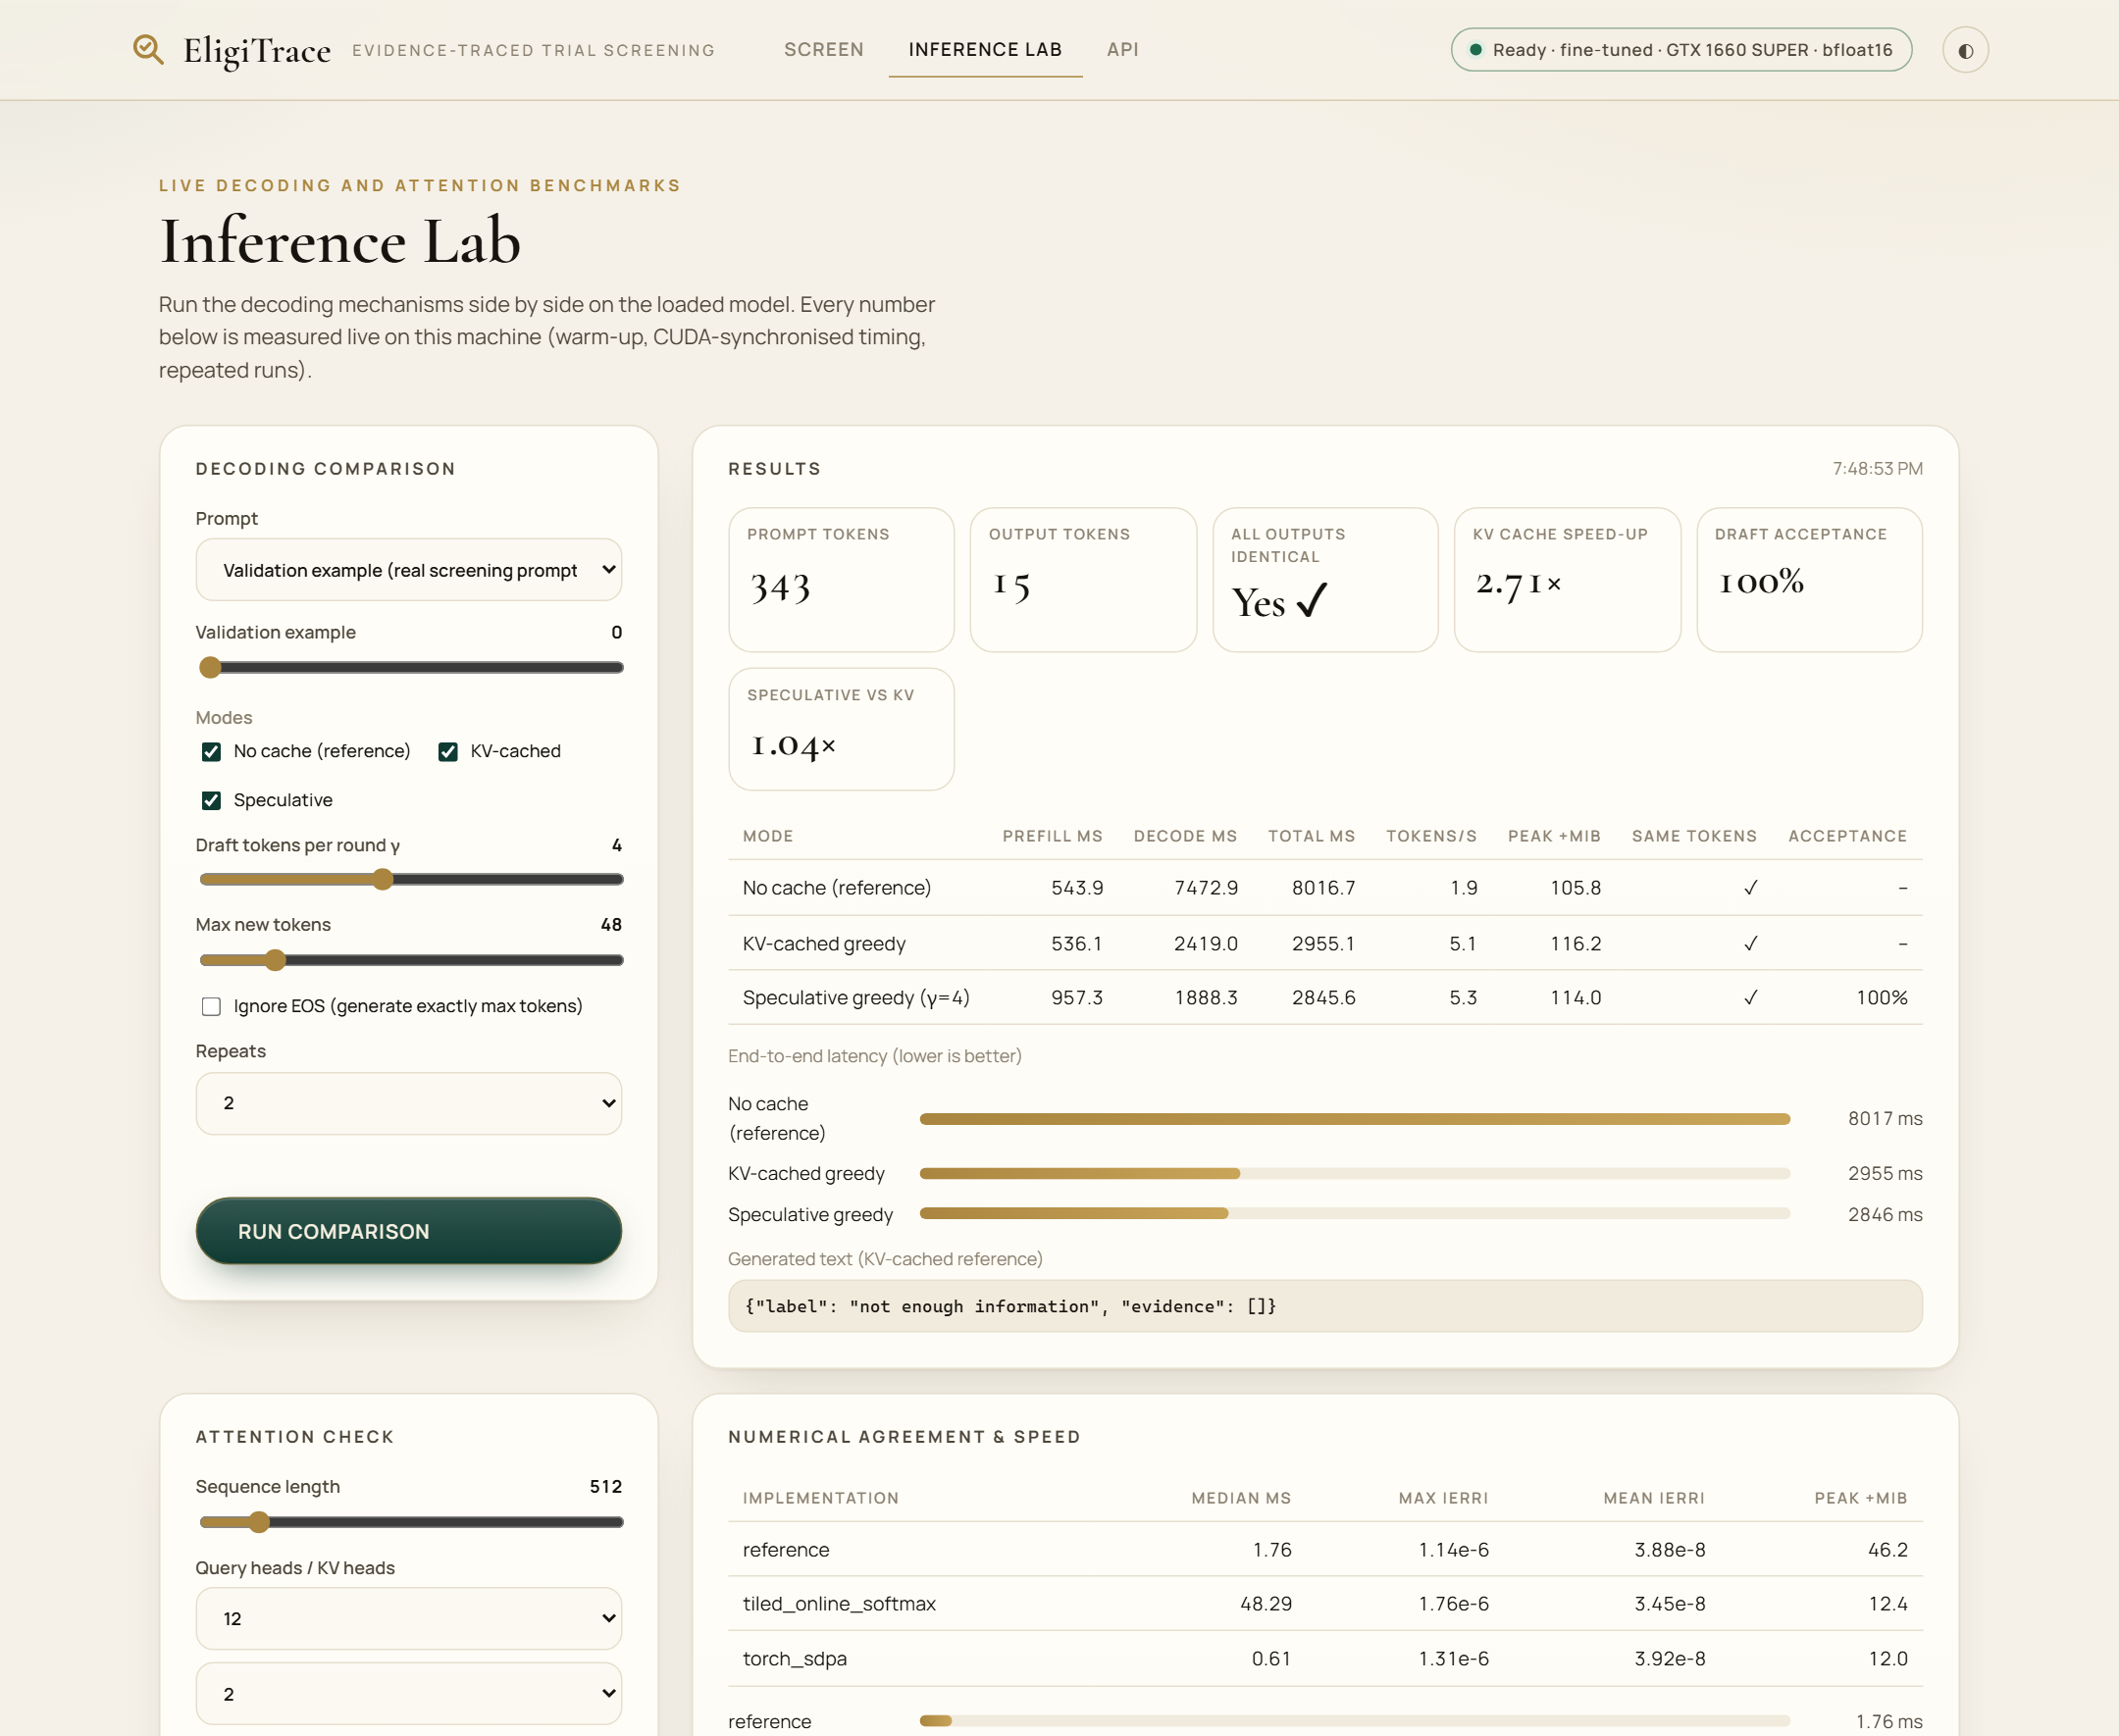
\includegraphics[width=0.49\linewidth]{screens/06_lab.png}\hfill
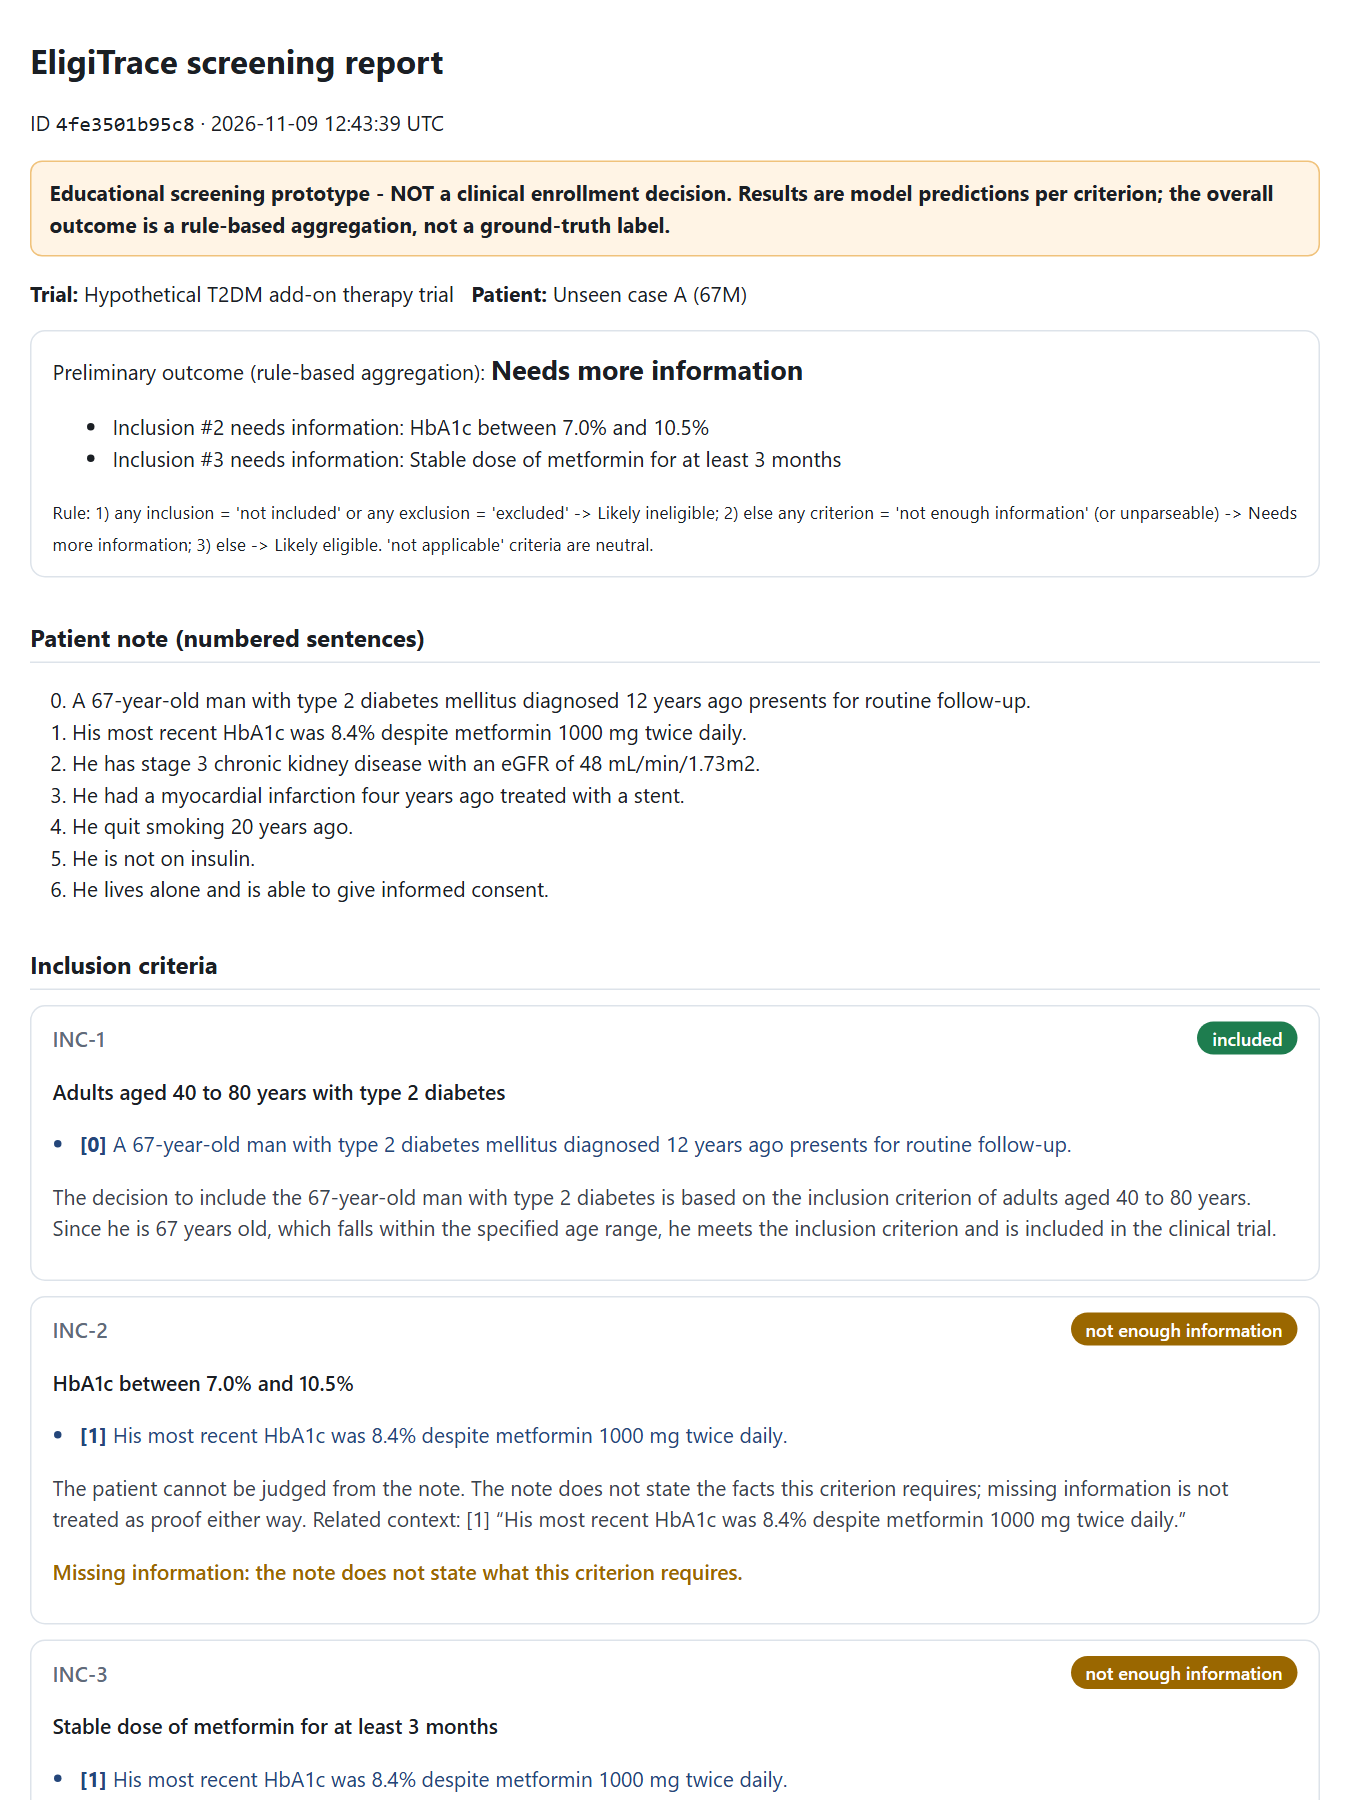
\includegraphics[width=0.49\linewidth]{screens/04_report.png}
\caption{\sys\ application. Top: input of an unseen note and criteria (left), and criterion results with
highlighted evidence, grounded rationales and the rule-based outcome (right). Bottom: Inference Lab with live
decoder and attention comparisons (left), and the exported report with provenance (right).}
\label{fig:app}
\end{figure*}
